
%%%%%%%%%%%%%%%%%%%%%%%%%%%%%%%%%%%%%%%%%%%%%%%%%%%%%%%%%%%%%%%%%%%%%%%%%%%%%%%%
%% BEFORE YOU START: 
%%
%% 1. Rename the paper.tex file into your paper name. Use the bibtex key policy 
%%    for the naming convention (see end of this file)
%%
%% 2. Change line 3 in the Makefile from "TARGET=paper" to "TARGET=name-of-tex-file"
%%
%%%%%%%%%%%%%%%%%%%%%%%%%%%%%%%%%%%%%%%%%%%%%%%%%%%%%%%%%%%%%%%%%%%%%%%%%%%%%%%%

\documentclass[letterpaper, 10 pt, conference]{ieeeconf}  % Comment this line out if you need a4paper
\IEEEoverridecommandlockouts                              % This command is only needed if
\overrideIEEEmargins                                      % Needed to meet printer requirements.

\usepackage{graphics}    % for pdf, bitmapped graphics files
\usepackage{times}       % assumes new font selection scheme installed
\usepackage{amsmath}     % assumes amsmath package installed
\usepackage{amssymb}     % assumes amsmath package installed
\usepackage{graphicx}
\usepackage{algorithm}
\usepackage[noend]{algpseudocode}
\usepackage{xcolor}

%% Align last page but causes error on some machines (such as OSX), so don't use for now.
%%\usepackage{flushend}

%% Style hacks to save space
%\setlength{\textfloatsep}{1.5em}
%\setlength{\dbltextfloatsep}{1.5em}
%\usepackage[font=small]{caption}

%% Key definitions for text elements. USE THEM
\def\secref#1{Sec.~\ref{#1}}
\def\figref#1{Fig.~\ref{#1}}
\def\tabref#1{Tab.~\ref{#1}}
\def\eqref#1{Eq.~(\ref{#1})}
\def\algref#1{Alg.~\ref{#1}}

\newcommand\etal{\emph{et al.}}

\usepackage{amsopn}


\newcommand{\bJidx}[1]{\ensuremath{\mathbf{J}^{[#1]}}}
\newcommand{\cose}{\mathrm{cose}}
\newcommand{\bzidx}[1]{\mathbf{z}^{[{#1}]}}
\newcommand{\bxidx}[1]{\mathbf{x}^{[{#1}]}}
\newcommand{\bhidx}[1]{\mathbf{h}^{[{#1}]}}
\newcommand{\bOmegaidx}[1]{\mathbf{\Omega}^{[{#1}]}}
\newcommand{\bSigmaidx}[1]{\mathbf{\Sigma}^{[{#1}]}}
\newcommand{\bHidx}[1]{\mathbf{H}^{[{#1}]}}

\newcommand{\bv}{\mathbf{v}}
\newcommand{\bl}{\mathbf{l}}
\newcommand{\bt}{\mathbf{t}}
\newcommand{\bo}{\mathbf{o}}
\newcommand{\bM}{\mathbf{M}}
\newcommand{\bL}{\mathbf{L}}
\newcommand{\bA}{\mathbf{A}}
\newcommand{\bB}{\mathbf{B}}
\newcommand{\bE}{\mathbf{E}}
\newcommand{\bK}{\mathbf{K}}
\newcommand{\bC}{\mathbf{C}}
\newcommand{\bG}{\mathbf{G}}
\newcommand{\bH}{\mathbf{H}}
\newcommand{\bI}{\mathbf{I}}
\newcommand{\bP}{\mathbf{P}}
\newcommand{\bX}{\mathbf{X}}
\newcommand{\bZ}{\mathbf{Z}}
\newcommand{\bR}{\mathbf{R}}
\newcommand{\bS}{\mathbf{S}}
\newcommand{\bU}{\mathbf{U}}
\newcommand{\bV}{\mathbf{V}}
\newcommand{\bT}{\mathbf{T}}
\newcommand{\bpi}{\mathbf{\pi}}
\newcommand{\btl}{\mathbf{tl}}
\newcommand{\bbr}{\mathbf{br}}


\newcommand{\iD}{\mathbf{D}}
\newcommand{\iN}{\mathbf{N}}
\newcommand{\iI}{\mathbf{I}}

\newcommand\norm[1]{\left\lVert#1\right\rVert}

\newcommand{\bzridx}[1]{\ensuremath{\mathbf{z}^{({#1})}}}
\newcommand{\bxridx}[1]{\mathbf{x}^{({#1})}}
\newcommand{\bhridx}[1]{\mathbf{h}^{({#1})}}

\newcommand{\bJ}{\mathbf{J}}
\newcommand{\bZero}{\mathbf{0}}

\newcommand{\cS}{\mathcal{S}}
\newcommand{\cG}{\mathcal{G}}
\newcommand{\cE}{\mathcal{E}}
\newcommand{\cC}{\mathcal{C}}
\newcommand{\cSM}{\mathcal{SM}}
\newcommand{\cR}{\mathcal{R}}
\newcommand{\cM}{\mathcal{M}}
\newcommand{\cP}{\mathcal{P}}
\newcommand{\cL}{\mathcal{L}}
\newcommand{\cD}{\mathcal{D}}
\newcommand{\cZ}{\mathcal{Z}}
\newcommand{\cX}{\mathcal{X}}
\newcommand{\range}[3]{#1_{#2:#3}}


\newcommand{\ba}{\mathbf{a}}
\newcommand{\bb}{\mathbf{b}}
\newcommand{\bc}{\mathbf{c}}
\newcommand{\bd}{\mathbf{d}}
\newcommand{\be}{\mathbf{e}}
\newcommand{\ec}{\mathbf{e}}
\newcommand{\bm}{\mathbf{m}}
\newcommand{\bg}{\mathbf{g}}
\newcommand{\Dim}{\mathrm{Dim}}

\newcommand{\bs}{\mathbf{s}}
\newcommand{\bx}{\mathbf{x}}
\newcommand{\by}{\mathbf{y}}
\newcommand{\br}{\mathbf{r}}
\newcommand{\bz}{\mathbf{z}}
\newcommand{\bu}{\mathbf{u}}
\newcommand{\bn}{\mathbf{n}}
\newcommand{\bh}{\mathbf{h}}
\newcommand{\bff}{\mathbf{f}}
\newcommand{\bp}{\mathbf{p}}
\newcommand{\bDelta}{\mathbf{\Delta}}
\newcommand{\bGamma}{\mathbf{\Gamma}}
\newcommand{\bDeltaalpha}{\mathbf{\Delta \alpha}}
\newcommand{\bDeltar}{\mathbf{\Delta r}}
\newcommand{\bDeltax}{\mathbf{\Delta x}}
\newcommand{\bDeltaX}{\mathbf{\Delta X}}
\newcommand{\bDeltat}{\mathbf{\Delta t}}
\newcommand{\bDeltaR}{\mathbf{\Delta R}}
\newcommand{\tTov}{\mathrm{t2v}}
\newcommand{\vTot}{\mathrm{v2t}}

\newcommand{\bO}{\mathbf{O}}

\newcommand{\defeq}{=}


\newcommand{\bmu}{\mathbf{\mu}}
\newcommand{\bnu}{\mathbf{\nu}}
\newcommand{\bSigma}{\mathbf{\Sigma}}
\newcommand{\bOmega}{\mathbf{\Omega}}
\newcommand{\bLambda}{\mathbf{\Lambda}}

\newcommand{\mat}[1]{#1}
\newcommand{\mbf}[1]{\mathbf{#1}}
\newcommand{\defn}[1]{\emph{#1}}

\newcommand{\mysum}{\sum}
\newcommand{\myprod}{\prod}
\newcommand{\eq}{=}
\newcommand{\pv}{\mathrm{P}}
%\newcommand{\implies}{\Rightarrow}
\newcommand{\Parents}{\mathrm{Parents}}
\newcommand{\rj}{\mathrm{j}}
\newcommand{\proj}{\mathrm{proj}}
\DeclareMathOperator*{\argmax}{argmax}
\DeclareMathOperator*{\argmin}{argmin}
\DeclareMathOperator*{\atantwo}{atantwo}

\newcommand{\mR}{\mathbb{R}}
\newcommand{\mN}{\mathbb{N}}
\newcommand{\mC}{\mathbb{C}}



%% Other useful macros
\newcommand\todo[1]{\textbf{[TODO: #1}]}

%% Some math definition
\def\argmax{\mathop{\rm argmax}}
\def\argmin{\mathop{\rm argmin}}
\newcommand{\bigO}[1]{$\mathcal{O}(#1)$}


%%%%%%%%%%%%%%%%%%%%%%%%%%%%%%%%%%%%%%%%%%%%%%%%%%%%%%%%%%%%%%%%%%%%%%%%%%%%%%%%
\title{\LARGE \bf A Complete System for Semantic Perception, Mapping and Exploration}

\author{Federico Nardi \and Roberto Capobianco \and Daniele Nardi% <-this % stops a space
  \thanks{All authors are with the Sapienza University of Rome, 
  Department of Computer, Control, and Management Engineering  "Antonio Ruberti", Rome, Italy. }%
  %\thanks{This work has partly been supported by ...
  %the EC under the grant number H2020-ICT-644227-Flourish. 
  %the EC under the grant number H2020-ICT-645403-RobDREAM.
  %the DFG under the grant number FOR~1505: Mapping on Demand.
  %}%
}

\begin{document}
\maketitle
\thispagestyle{empty}
\pagestyle{empty}


%%%%%%%%%%%%%%%%%%%%%%%%%%%%%%%%%%%%%%%%%%%%%%%%%%%%%%%%%%%%%%%%%%%%%%%%%%%%%%%%
\begin{abstract}
  %
  % WHY is it relevant
  \emph{1-2 not too long sentences clearly answering the WHY question.}
  
  % WHICH PROBLEM are we adressing
  In this paper, we present a ....  . 

  % HOW is our approach special, WHAT are we actually doing, and WHAT IS NEW
  Our approach ... \emph{(complete, around 2-3 sentences)}
 
  %% IMPLEMENTATION, EVALUATION, WHAT FOLLOWS 
  We implemented our approach using C++ and ROS and thoroughly tested
  it on .... \emph{(finish sentence)}. The experiments presented in
  this paper show that ... \emph{(finish sentence)}
\end{abstract}


%%%%%%%%%%%%%%%%%%%%%%%%%%%%%%%%%%%%%%%%%%%%%%%%%%%%%%%%%%%%%%%%%%%%%%%%%%%%%%%%
\section{Introduction}
\label{sec:intro}

In order to autonomously operate in human environments, robots need the ability to build and maintain an internal representation of their workspace. Traditional mapping techniques return a geometric model of the environment that can be used for computing distances to obstacles or finding paths toward goals. However, some manipulation and navigation tasks may require human level knowledge (e.g., objects/places categories, functions, properties, and so on) to be effectively executed, thus, requiring also the acquisition and modeling of semantic information.

%In recent years, the field of Semantic Mapping has experienced a rise in interest both from AI and Robotics communities. Traditional approaches propose custom solutions that usually work under limiting assumptions and are tailored to specific applications. In this work, we propose a general and complete semantic mapping system that allows to be effectively deployed in different 
%scenarios, paving the way to the next generation robotic applications.

The problem of building such a representation of the environment can be addressed by facing three aspects: 1) processing sensor data to extract geometric and semantic information, 2) modeling these information in a suitable representation that support task execution and 3) planning the robot motion to maximize the extraction of such information. In the past, these aspects have been separately addressed by researchers who mainly focused on one of them assuming others were already solved or not relevant.

In this work, we propose a general and complete semantic mapping system that simultaneously aims at addressing in a unified framework the three above mentioned sub-problems. This allows our system to be effectively deployed in different scenarios, making a step towards the next generation robotic applications.

%% HOW & WHAT; already briefly mention what is novel (but go more in detail in the next paragraph)
{\color{blue}\emph{HOW: Third, explain briefly HOW your approach is special and then WHAT 
you do concretely.}}

\dots

\begin{figure}[ht]
  \centering
 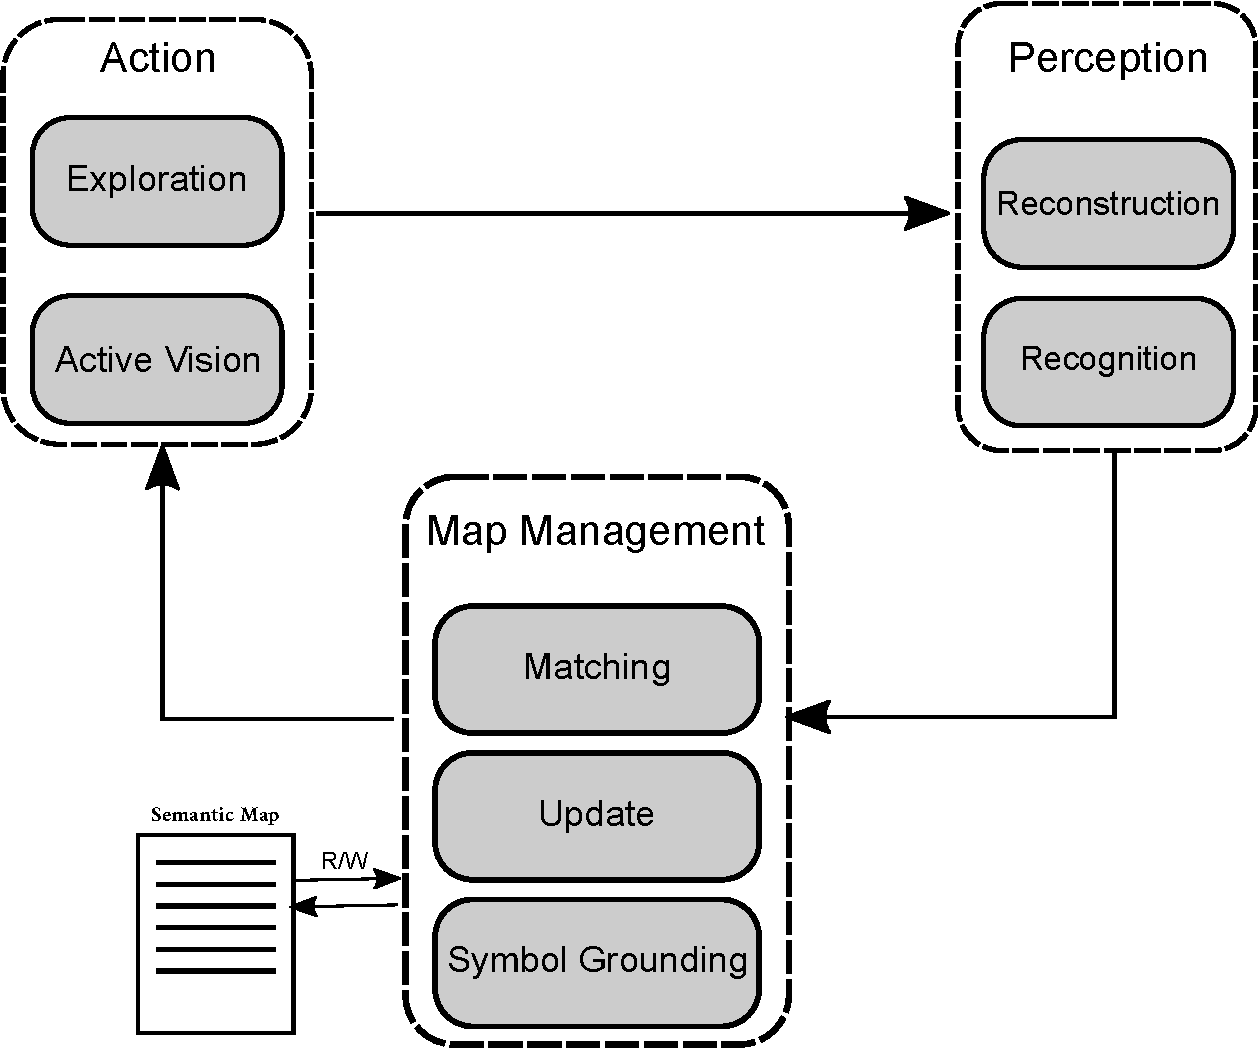
\includegraphics[width=0.99\linewidth]{pics/drawing-crop}
 \caption{Motivating Example. Provide a caption that lets the reader
   understand the image easily.  This image should be on top of the
   right column of page~1.}
  \label{fig:motivation}
\end{figure}

%% MAIN CONTRIBUTION & WHAT FOLLOWS FROM THAT
{\color{blue}\emph{Explain your contribution in one paragraph. Start that paragraph with:}}

The main contribution of this paper is a ....  We achieve this by
... This allows us to ... See \figref{fig:motivation} for an example.

The main contribution of this paper is a thorough study of literature related to Semantic Mapping with the aim of providing a template

%% CLAIMS (can be merged with main contribution)
{\color{blue}\emph{Claims: Explicitly state your claims in one paragraph using (i)
  ..., (ii) ..., (iii) ... and, if useful, spell out the key
  assumptions. You can do that here or merge the caims with the
  previous paragraph about the main contribution. For example:}}

In sum, we make N key claims, which are are the follwing:
Our approach is able to
%
(i) ..., 
%
(ii) ..., 
%
(iii) ... and,
%
(iv) . 
% 
These N claims are backed up by the paper and especially 
our experimental evaluation.


%%%%%%%%%%%%%%%%%%%%%%%%%%%%%%%%%%%%%%%%%%%%%%%%%%%%%%%%%%%%%%%%%%%%%%%%%%%%%%%%
\section{Building a Semantic Representation of the Environment}
\label{sec:map}

A semantic map is a collection of elements

\begin{equation}
\cSM = \{ \bE_1 \dots \bE_N \},
\end{equation}

where each element $\bE_i = < \cG_i, \cS_i>$ represents an object in the scene and is characterized by geometric and semantic information.

\subsection{Geometric Information $\cG$}

The former describes the geometric properties of each element of the map. To fully qualify an element geometry we make us of:
\begin{itemize}
	\item {\bf Pose3D}: $\bX = [ \bR | \bt] \in SE(3)$, it's expressed in a global reference system $\cR^G$ and defines the element reference system $\cR^E$.
	\item {\bf Size3D}: $\bS = <\bL ,\bU> \in \mathbf{R}^3 $, it's represented by two 3D vectors that define the smallest \emph{axis-aligned} bounding box that contains the whole element.
	\item {\bf Representation3D}: $\bM$, a digital model of the element surface (e.g. point cloud, mesh and so on).
\end{itemize}

\subsection{Semantic Information $\cS$}

While, the latter describes the semantic information of each elements of the map through the following properties:
\begin{itemize}
	\item {\bf Type}: $t \in \cL$, the element category. It's selected by the recognition module among the possible semantic labels $\cL = \{l_1 \dots l_M \}$.
	\item {\bf Properties:} $\bP = \{ p_1 \dots p_K \}$, other semantic information related to the element, e.g. relationships with other elements, physical properties, functionalities, and so on. 
\end{itemize}   

\subsection{Semantic Mapping Process}

To build such a representation, the semantic mapping process can be decomposed in three steps (see~\figref{fig:system}): \emph{1) perception}, the output of visual and range sensors is processed to extract information for recovering the structure and objects/places categories of the scene; \emph{2) map management}, these information is used to update the current belief about the state of the environment; \emph{3) action}, next pose for the robot is computed in order to improve its representation of the environment. In the remainder, we will present a detailed description of each of these sub-problems along with our proposed implementation.

\begin{figure}[ht]
	\centering
	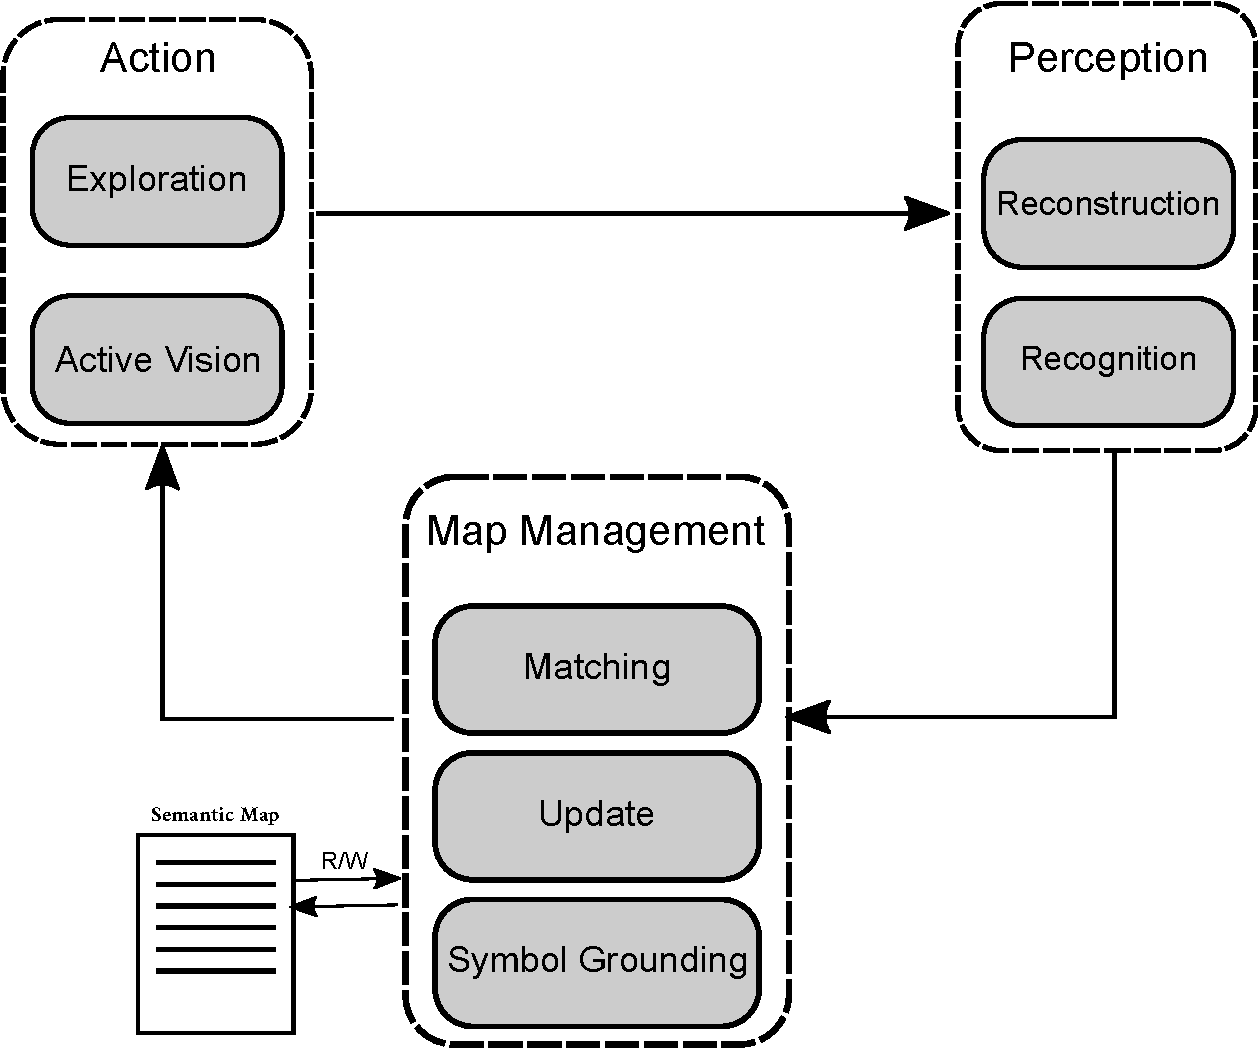
\includegraphics[width=0.99\columnwidth]{pics/drawing-crop}
	\caption{A caption that makes you understand the image easily.}
	\label{fig:system}
\end{figure}

%%%%%%%%%%%%%%%%%%%%%%%%%%%%%%%%%%%%%%%%%%%%%%%%%%%%%%%%%%%%%%%%%%%%%%%%%%%%%%%%
\section{Perception}
\label{sec:perception}


The perception module takes as input sensor measurements $\cS = \{ \bs_1 \dots \bs_T \}$ acquired by the robot during exploration and returns a list of elements $\cE = \{ \bE_1 \dots \bE_N \}$.

This is the core component of every semantic mapping system and several approaches have been proposed. A possible categorization of these methods can take into account the way in which \emph{reconstruction} and \emph{recognition} are combined to obtain the final output.

In this view, a first class of methods may fit under the definition of "purely semantic". The reason is that these methods focus only on the extraction of semantic information about objects/places from sensory data, assuming that no reconstruction is needed. Despite based on recognition, these methods don't build a map of the environment and, thus, are very limited in practice.

Traditional semantic mapping approaches work by "serializing" reconstruction and recognition. That is, they first build a geometric model of the environment and, subsequently, use this model to extract semantic information. Contrary to the previous ones, these works address the map management problem, however, this is typically done \emph{off-line} which may be unsuitable for many robotic applications.

That's why more recent methods perform reconstruction and recognition "in parallel". This approach is motivated by recent advances in both investigation fields, namely, dense 3D SLAM with RGB-D sensors and image analysis with Convolutional Neural Networks (CNNs). However, since the map representations built with the SLAM system describe the environment surface as a set of low-level geometric primitives (i.e., points, edges, voxels), how this information can be used by the robot still remains an open issue.

\subsection{Reconstruction}

Consists in processing sensor measurements $\cS$ to recover both the set of robot poses $\cX = \{ \bx_1 \dots \bx_T \}$ and a digital representation of the environment $\cM$. In robotic applications, it is mainly performed by addressing the "Simultaneous Localization and Mapping" (SLAM) problem. The advent of affordable RGB-D sensors gave a strong impulse in this investigation field and the proposed solutions can be categorized according to how the scene surface is represented \cite{cadena2016ieeetransrob}.

In the majority of SLAM methods, the scene is represented by a set of sparse 3D landmarks that correspond to relevant features in the environment (e.g. edges, corners) \cite{mur2015ieeetransrob}.	These methods are attractive because they're based on a lightweight formulation and still they're effective in accurately localizing the robot, but they provide a rather poor representation of the environment since they tend to filter out portions with less features.

A different approach is to describe the 3D geometry by means of large unstructured set of points (i.e., point clouds), which are obtained by nowadays easily available RGB-D cameras. Contrary to landmark-based methods, there are also "direct" methods that estimate the trajectory of the robot and a 3D model directly from the intensity values and/or depth values of all the image pixels \cite{newcombe2011ICCV,steinbrucker2011real}. This type of representation allows to better infer the structure of the scene but it still may contain artifacts in some portions of the environment due to the uneven sensor sampling density.

A reasonable choice to overcome this limitation is to introduce structured representations, such as the ones used in Computer Graphics for Surface Reconstruction \cite{berger2014state}. These are called "boundary representations", since they define 3D objects in terms of their surface boundary. In general, b-reps can be classified as: curve-based representations (NURBS or B-Spline), mesh representations (triangulated surfaces) and implicit representations (level-set surfaces). The latter was investigated in the work of Newcombe et al. \cite{newcombe2011kinectfusion} and received much interest from the SLAM community thanks to its representation power. The main drawback is the not negligible amount of memory required also in the case of small scale scenes. This limits considerably the scalability of this method and the development of optimized techniques for large-scale environments is an open issue \cite{kahler2015very,vespa2018efficient}.

All the representations mentioned so far describe the environment surface by means of low-level features. Another approach, proposed in the seminal work by Moreno~\etal \cite{salas2013CVPR}, is to investigate higher level object-based representations, where the map is made of objects and solid shapes as it is the case in Computer Aided Design (CAD).

\subsection{Recognition}

Consists in extracting subsets of sensory data (patterns) belonging to known objects and scenes categories and assign them the corresponding semantic label. Typically, in robotic applications input data can be of two types: \emph{raw}, recognition is performed directly on sensor data and each time the sensor returns a measurement; \emph{reconstructed}, recognition is performed on a scene obtained with reconstruction methods. The output of the recognition step consists in a list of detections $\cD = \{ \bd_1 \dots \bd_N \}$, that, in general, may contain just one element (classification) or a sequence of them (detection, segmentation). Each entry in the detection list $\bd_i$ is characterized by: 
\begin{itemize}
	\item {\bf Semantic Label}: that identifies the semantic category of the detection. 
	\item {\bf Spatial Location}: that express the position of the detection w.r.t. the reference system of the input data.
\end{itemize}

Recognition can be decomposed into sub-tasks, depending on the information one is interested to extract from the input data. These sub-tasks can be organized on a progression that goes from coarse to fine grained inference.

Image classification is the task of assigning a semantic label to an input image from a fixed set of categories. Ulrich and Nourbakhsh \cite{ulrich2000icra} propose an appearance-based place recognition system for topological localization. They use colour histogram features \cite{swain1991ijcv} and a simple voting scheme for nearest-neighbor matching. In a similar fashion, Torralba \etal~\cite{torralba2003context} derive an hidden Markov model (HMM) for place recognition and new place categorisation based on the global statistic feature retrieved from texture \cite{oliva2001ijcv}. In contrast, Lisin \etal~\cite{lisin2005cvpr} propose to model classes of images as a probability distribution over local features, in order to be combined with global features. This method has proven to perform well in applications where a rough segmentation of objects is available.

Object detection consists of making a prediction not only of object categories but also of their spatial locations. A seminal work can be considered that of Viola and Jones \cite{viola2004ijcv}, who proposed a fast and robust face detection. Their method makes use of Haar-like features \cite{papageorgiou1998iccv} to search for likely face candidates, which can then be refined using a cascade of more expensive but selective detection algorithms \cite{freund1997jcss}. Likewise, a well-known example of pedestrian detection has been proposed by Dalal and Triggs \cite{dalal2005cvpr}, who use a set of overlapping Histogram of Oriented Gradients (HOG) descriptors fed into a Support Vector Machine (SVM) \cite{cortes1995support}.

Image segmentation is the task of finding groups of pixels that possess some "similarity" and is one of the oldest and most widely studied problems in computer vision.
Early techniques focus on local region merging and splitting \cite{ohlander1978picture,brice1970scene}, while, more recent algorithms often optimize some global criterion, such as intra-region consistency and inter-region boundary lengths or dissimilarity \cite{comaniciu2002pami,shi2000pami,felzenszwalb2004ijcv,chan2001ip,osher1988jcp}. 

Despite the popularity of the presented methods, a recent breakthrough in scene understanding has been the adoption of Convolutional Neural Networks (CNNs) \cite{garcia2017review}. Krizhevsky \etal in \cite{krizhevsky2012nipsjournal} present the pioneering deep CNN that, despite its simplicity, won the Imagenet 2012 classification challenge with wide margin on the closest competitor. Similarly, different object detection methods based on deep neural netowrks have shown to outperform the state-of-the-art \cite{redmon2016cvpr,erhan2014cvpr,liu2016eccv}. Consequently, the capabilities of such networks have been also investigated in pixel-level labeling problems like semantic segmentation. In this context, a milestone is the work of Long \etal~\cite{long2015cvpr} who transformed existing classification models (\cite{simonyan2014very,szegedy2015cvpr}) into fully convolutional ones to output spatial maps instead of classification scores. One of the main reason behind its popularity is that, with this approach, CNNs can be trained end-to-end and efficiently learn to make dense predictions with inputs of arbitrary size.
	
%%%%%%%%%%%%%%%%%%%%%%%%%%%%%%%%%%%%%%%%%%%%%%%%%%%%%%%%%%%%%%%%%%%%%%%%%%%%%%%%
\section{Map Management}
\label{sec:mapman}

The map manager has the task of incrementally updating the semantic map with new information coming from the perception module. 

The input to the map management module is the list of elements $\cSM^R$ returned by the perception module, where the superscript $R$ denotes that the elements are expressed in the robot local reference frame. After matching the elements in $\cSM^R$ with those already seen and contained in $\cSM^G$, where the superscript $G$ denotes that the elements are expressed in the global reference frame, the incoming information is inserted in the semantic map, in order to return an up to date version of $\cSM^R$.

Existing approaches may be classified according to two different aspects: whether the semantic map is built after all sensor measurements have been acquired (\emph{off-line}) or during the exploration phase (\emph{frame-by-frame}) and whether the elements in the semantic map are linked to predicates in a Knowledge Base (KB) (\emph{with-KB}) or not (\emph{without-KB}).

\subsection{Matching}

In order to update the semantic map when new sensor measurements are acquired, it's necessary to maintain a correspondence between the objects being observed and their internal representations. This is done by finding the set of correspondences $\cC = \{\bc_1 \dots \bc_K\}$ between elements in the robot local map $\cSM^R$ and elements in the global map $\cSM^G$. A correspondence between two elements can be assessed through a similarity measure $d(\bE_i^R,\bE_j^G)$. The $k$-th correspondence $\bc^{i,j}_k \eq <\bE_i^R,\bE_j^G>$ establishes that the $j^{th}$ element $\bE_j^G$ in the global map is the "closest" to the $i^{th}$ element $\bE_i^R$ in the local map. That is:
\begin{equation}
\bE_i^R = \argmin_{\bE_i} \, d(\bE_i^R,\bE_j^G)
\end{equation} 

Possible approaches are:
\begin{itemize}
	\item $\dots$
\end{itemize}

\subsection{Update}

Consists in inserting new information coming from the perception module in the environment representation of the robot in order to return an updated map.

This module processes the set of correspondences $\cC$ and, for each correspondence $\bc^{i,j}_k$, executes one of two operations:
\begin{itemize}
	\item $d(\bE_i^R,\bE_j^G) \leq d_{th}$: $\bE_i^R$ matches with $\bE_j^G$ $\rightarrow$ Merge the two elements.
	\item $d(\bE_i^R,\bE_j^G) > d_{th}$: $\bE_i^R$ has not been already seen $\rightarrow$ Add the element to the map.
\end{itemize}

Possible approaches are:
\begin{itemize}
	\item {\bf Bayesian:} the update of an element considers past observations.
	\item {\bf Context aware:} the update of an element considers also spatial relations with other elements.
\end{itemize}

\subsection{Symbol Grounding}

\begin{itemize}
	\item Consists of linking symbols, the elements in $\cSM^G$, to concepts in a Knowledge Base (KB).
	\item Possible approaches are:
	\begin{itemize}
		\item $\dots$
	\end{itemize}
\end{itemize}	

%%%%%%%%%%%%%%%%%%%%%%%%%%%%%%%%%%%%%%%%%%%%%%%%%%%%%%%%%%%%%%%%%%%%%%%%%%%%%%%%
\section{Exploration}
\label{sec:exploration}

It consists in planning sensor motion in order to recover as much as possible geometric and/or semantic information of the environment. The input to the exploration module is the current belief about the state of the world, i.e., map, which contains the robot knowledge about the environment and robot pose, that represents the estimate of its position in it. This information is then used to compute a motion trajectory for the exteroceptive sensors mounted on the robot that allows to improve the reconstruction of the scene and/or the recognition of objects and places.

%Application:
%
%\begin{itemize}
%	\item navigation
%	\item reconstruction
%	\item recognition
%\end{itemize}

\subsection{Active Vision}

%\begin{itemize}
%	\item difference between considering the whole space of possible viewpoints w.r.t. choosing a fixed subset of them
%	\item most of the approaches only perform a reconstruction of the environment without explicitly model the single objects perceived by the robot in its internal representation
%	\item one big limitation of many methods is that they segment the scene geometrically
%\end{itemize}

For navigation applications, a common solution is to adopt frontier-based strategies. In an occupancy grid, frontiers are sets of adjacent free cells that have at least a neighboring cell whose occupancy is unknown. Once frontiers are detected on the map, a score is assigned to each of them depending on some criteria (e.g. information gain, distance and bearing w.r.t the robot, traversability and so on) and the robot is directed towards the top scoring one. Another strategy to detect frontiers is based on randomized search techniques that sample the robot configuration space and find traversable paths to expand the mapped area. 

Typical manipulation applications require the reconstruction of accurate 3D models of the objects to be manipulated. This problem is addressed by automatic view selection or Next Best View (NBV), in order to ensure that the entire (visible) surface of an object will be scanned, preferably minimizing the number of scan acquisitions. 

In case of a mobile manipulator with an eye-in-hand sensor facing the target object, the next best view can be determined by search or optimization techniques. These methods perform a volumetric reconstruction of the scene that is used for view evaluation according to one or more criteria, e.g., information gain, motion cost, surface overlap and so on. In this setting, the reconstruction is considered completed when it is no more possible to find a view that senses unknown space. 

Another possible choice for a stop criterion is to leverage semantic information. This approach may be useful under the assumption of several objects to reconstruct or in case active vision should improve object recognition. As before, the volumetric reconstruction is performed for view evaluation, in addition, the results of a 3D object recognition module may be interpreted to evaluate if the representation of the environment is accurate enough.




%%%%%%%%%%%%%%%%%%%%%%%%%%%%%%%%%%%%%%%%%%%%%%%%%%%%%%%%%%%%%%%%%%%%%%%%%%%%%%%%
\section{Our Approach}
\label{sec:main}

\emph{Describe your approach. It is okay to divide the main section
  into a few subsection (e.g., 2-4 subsections).}


Use equations in the style of
\begin{eqnarray}
\label{eq:nameeqn}
  p(x) &=& \alpha + \beta.
\end{eqnarray}

In \eqref{eq:nameeqn}, the term~$\alpha$ refers to ...

\emph{A few comments:
\begin{itemize}
	\item Add a tilde (\textasciitilde) in front of inline math (using \$) to avoid a line break.
	\item Add a tilde (\textasciitilde) in front of a cite to avoid a line break.
	\item Use the macros \textbackslash{}figref, \textbackslash{}tabref, \textbackslash{}secref, \textbackslash{}eqref for referencing
	\item Separate number and units using \textbackslash{}, for example 1\textbackslash{},m, which results in 1\,m
 \end{itemize}
}

%%%%%%%%%%%%%%%%%%%%%%%%%%%%%%%%%%%%%%%%%%%%%%%%%%%%%%%%%%%%%%%%%%%%%%%%%%%%%%%%
\section{Experimental Evaluation}
\label{sec:exp}

\emph{Repeat the main focus/objective with one sentence starting with:}
%
The main focus of this work is a  ..... 

\emph{Explain the reader that the experiments with support all claims
  (same list as in the intro!) starting the paragraph with:} 
%
Our experiments are designed to show the capabilities of our method and to
support our key claims, which are: 
%
(i)~..., 
%
(ii)~..., 
%
(iii)~..., and
%
(iv)~....

We furthermore provide comparisons to a popular method for ... as
proposed in~\cite{}.  We perform the evaluations on own datasets as
well as on publicly available ones.  Throughout all these experiments,
we set the key parameter of our approach to $X=1$ as this provided the
best performance as shown in \figref{fig:parameval}.

\emph{If needed (and only then!) say also a few words about the
  experimental setup, the datasets, and used parameters. You can use
  an own subsection if you want to put focus on that but often that is
  not needed.}

\emph{Note 1: It MUST be always crystal clear (a) WHY an experiment is
  there (e.g., to support a claim, to show that the approachis useful
  for real word systems, to show the performance, or to provide a
  baseline comparison), (b) WHAT it wants to show (which
  claim/property exactly), and (c) HOW it aims at showing this. This
  is ESSENTAIL for a good evaluation. Think about when BEFORE
  designing an experiment.}

\emph{Note 2: Start with the most important/impressive experiment
  first. Make this a key story of the paper. Keep the order of the
  claims, i.e., re-order claims in the intro/before if needed. }

%%%%%%%%%%%%%%%%%%%%%%%%
\subsection{Performance}

\emph{Start EVERY experiment with a similar start as the following
  sentence, explaining in the first sentence why you present the
  experiment and which claim it aims at supporting.}

%% First experiment - most impressive, important or the most important
%% claim supporting experments comes first.
The first experiment is designed to show the performance of our
approach and to support the claim that it is well-suited for ....


%% Second experiment - could be a comparison to a baseline methods,
%% quality analysis or similar
The second experiment is to support the claim that our approach is ...

%%%%%%%%%%%%%%%%%%%%%%%%
\subsection{Runtime}

%% Rumtime experiment - it is often one of the last experimemts unless
%% online processing / speed is the key contribution
The next set of experiments in designed to support the claim that our
approach runs fast enough to support online processing on the robot in
real time. We therefore tested our approach on ....

\tabref{tab:speed} summarizes the runtime results for .....  The
numbers support our third (check!) claim, namely that the computations
can be executed fast and in an online fashion.  On a mobile i5 CPU, we
achieve average frame rates of XXX\,Hz-XXX\,Hz depending on ... and
XXX\,Hz-XXX\,Hz on an i7 desktop computer.
 
\begin{table}
\caption{Average runtime and std.~dev.}
\centering
{\footnotesize
\begin{tabular}{|c|c|c|}
\hline
XXXX & mobile & desktop \\
 & i5 CPU 2.2\,GHz & i7 CPU 3.5 GHz\\
\hline
configA & 2.4\,ms~$\pm$~0.5\,ms~$\approx$~416\,Hz & 1.5\,ms~$\pm$~0.2\,ms~$\approx$~667\,Hz \\
configB & 4.4\,ms~$\pm$~1.2\,ms~$\approx$~227\,Hz & 2.6\,ms~$\pm$~0.5\,ms~$\approx$~385\,Hz \\
configC & 8.6\,ms~$\pm$~2.6\,ms~$\approx$~116\,Hz & 4.7\,ms~$\pm$~1.2\,ms~$\approx$~212\,Hz \\
\hline
\end{tabular}
}
\label{tab:speed}
\end{table}

%%%%%%%%%%%%%%%%%%%%%%%%
\subsection{XXX Analysis}

Finally, we aim at supporting our claim that ....

\emph{Briefly summarize the evaluation and what follows with approx. 2
  sentences.}  In summary, our evaluation suggests that our method
provides competitive .... At the same time, our method is fast enough
for online processing and has small memory demands. Thus, we supported
all our claims with this experimental evaluation.


%%%%%%%%%%%%%%%%%%%%%%%%%%%%%%%%%%%%%%%%%%%%%%%%%%%%%%%%%%%%%%%%%%%%%%%%%%%%%%%%
\section{Conclusion}
\label{sec:conclusion}

In this paper, we presented novel approach to.....  
Our approach operates ....  Our method exploits ....  
This allows us to successfully ...  
We implemented and evaluated our approach on different datasets
and provided comparisons to other existing techniques and supported
all claims made in this paper. The experiments suggest that ...


%%%%%%%%%%%%%%%%%%%%%%%%%%%%%%%%%%%%%%%%%%%%%%%%%%%%%%%%%%%%%%%%%%%%%%%%%%%%%%%%
% Future work only if it makes sense 
\emph{Future work: Use only if applicable -- but if so, use the
  following sentence to start:} 

Despite these encouraging results, there is further space for
improvements. For example, ...


%%%%%%%%%%%%%%%%%%%%%%%%%%%%%%%%%%%%%%%%%%%%%%%%%%%%%%%%%%%%%%%%%%%%%%%%%%%%%%%%
% Only if applicable
%\section*{Acknowledgments}
%We thank XXX for fruitful discussions and for ...

\bibliographystyle{plain}
\bibliography{robots}

\end{document}

%%%%%%%%%%%%%%%%%%%%%%%%%%%%%%%%%%%%%%%%%%%%%%%%%%%%%%%%%%%%%%%%%%%%%%%%%%%%%%%%
%% NOTES ON PAPER WRITING
%
% Rename the paper.tex file into your paper name. Use the bibtex key policy (see below)
%
% Use a Spell Checker with US English as spelling language
% 
% Use Academic Writing Check: https://github.com/devd/Academic-Writing-Check
%
% Use GIT for version control. Use our gitlab sever!
%
% Make sure your Makefile is working correctly and compiles the documents 
%
% All images go to the subfolder pics and reviews into the revoiews folder
%
% Make sure the source files for images are in the pics folder as well (unless they are huge)
%
%%%%%%%%%%%%%%%%%%%%%%%%%%%%%%%%%%%%%%%%%%%%%%%%%%%%%%%%%%%%%%%%%%%%%%%%%%%%%%%%


%%%%%%%%%%%%%%%%%%%%%%%%%%%%%%%%%%%%%%%%%%%%%%%%%%%%%%%%%%%%%%%%%%%%%%%%%%%%%%%%
%% NOTES ON BIB ENTRIES
%
% Bibtex Key Policy
%
%    All in lower case
%    Use the key structure: <lastnamefirstauthor><2 digit year><conference/journal><extra>
%    Use <extra>:
%        for workshops: -ws,
%        for multiple papers: -a, -b, -c, ... ordered by title in alphabetical order
%        additionally add -a, -b, -c, ... ordered by title in alphabetical order in case of multiple workshops
%    Examples: stachniss08icra, stachniss08icra-ws, stachniss08icra-a, stachniss08icra-b
%    Use the bibtex key also at the filename for the paper, e.g., stachniss08icra.pdf
%
% Bibtex Entries
%
%    Use strings for conferences and journal name in order to keep obtain consistent entries
%    Use the identical abbreviations for conference name, e.g., “Proc. of the IEEE Int. Conf. on Robotics and Automation (ICRA)”
%    Avoid adding location in addition to the city or street of the conference.
%    Use doi for the official document on the publisher webpage. 
%    Abbreviate the first name of the authors, e.g., C. Stachniss instead of Cyrill Stachniss
%    In case of a first name and a middel name, use no space between them, e.g., C.J. Stachniss
%%%%%%%%%%%%%%%%%%%%%%%%%%%%%%%%%%%%%%%%%%%%%%%%%%%%%%%%%%%%%%%%%%%%%%%%%%%%%%%%


